\chapter[Story Board]{Story Board}
\label{chap:storyBoard}
	
	A história se passa no cotidiano de Samuel, um estudante da Universidade de Brasília - UnB. Durante o semestre, Samuel sempre que vai a alguma consulta com a coordenadora de seu curso, encontra uma fila de alunos aguardando o mesmo atendimento o que acaba gerando muita insatisfação para Samuel, pois ele perdia um tempo significativo na fila de espera, podendo estar fazendo outras atividades no mesmo tempo. 

	A coordenadora do curso de Samuel observando as dificuldades dos alunos em ter um atendimento com ela, resolver construir um aplicativo no qual era possível fazer um agendamento prévio para os alunos que desejam consultar-se com ela. Então, após o desenvolvimento do aplicativo, a coordenadora disponibilizou por e-mail o novo aplicativo desenvolvido. 
	
	Samuel ao receber o e-mail, resolve testar o aplicativo fazendo seu cadastro e agendando um atendimento com a coordenadora de seu curso. Ao chegar na sala da coordenadora, ela o cumprimenta pelo nome, pois o aplicativo disponibiliza a agenda de atendimento para a coordenadora com os nomes dos alunos agendados e suas respectivas datas e horários. Samuel, muito contente, fica satisfeito pois não necessitou pegar fila alguma para seu atendimento. 

	\newpage

	\begin{figure}[h]
		\centering
		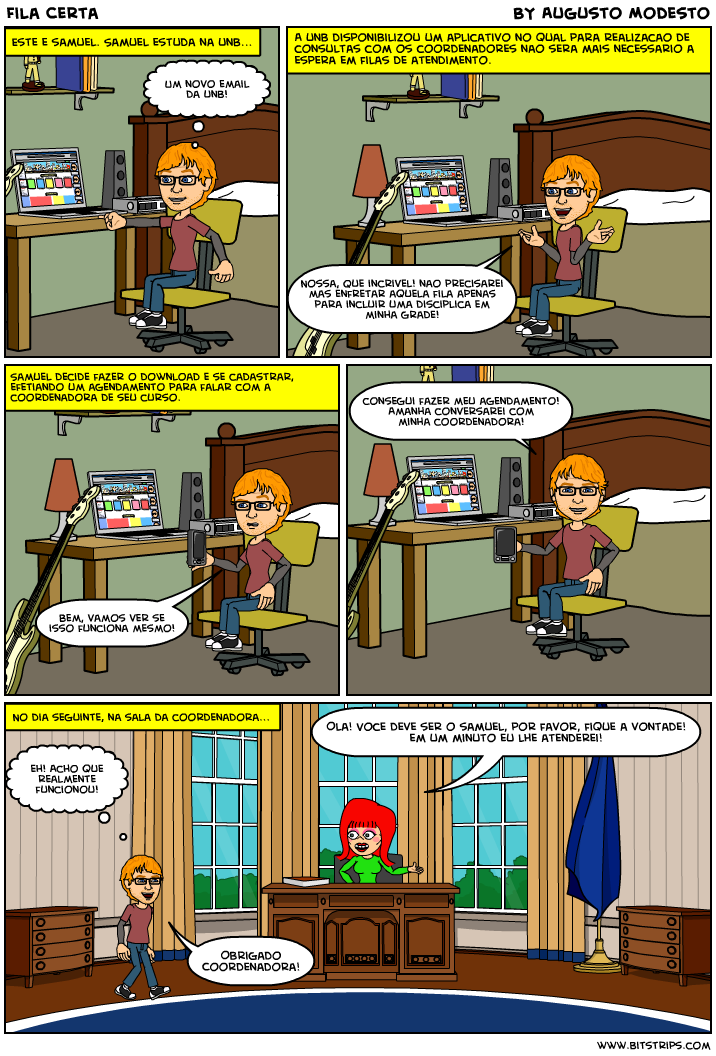
\includegraphics[scale=0.6]{story_board}
		\caption[Story Board para aplicação]{Story Board para aplicação.}
		\label{fig:metas_Experiencia_Usuario}
	\end{figure}